\let\negmedspace\undefined
\let\negthickspace\undefined
\documentclass[journal]{IEEEtran}
\usepackage[a5paper, margin=10mm, onecolumn]{geometry}
%\usepackage{lmodern} % Ensure lmodern is loaded for pdflatex
\usepackage{tfrupee} % Include tfrupee package

\setlength{\headheight}{1cm} % Set the height of the header box
\setlength{\headsep}{0mm}     % Set the distance between the header box and the top of the text

\usepackage{gvv-book}
\usepackage{gvv}
\usepackage{cite}
\usepackage{amsmath,amssymb,amsfonts,amsthm}
\usepackage{algorithmic}
\usepackage{graphicx}
\usepackage{textcomp}
\usepackage{xcolor}
\usepackage{txfonts}
\usepackage{listings}
\usepackage{enumitem}
\usepackage{mathtools}
\usepackage{gensymb}
\usepackage{comment}
\usepackage[breaklinks=true]{hyperref}
\usepackage{tkz-euclide} 
\usepackage{listings}
% \usepackage{gvv}                                        
\def\inputGnumericTable{}                                 
\usepackage[latin1]{inputenc}                                
\usepackage{color}                                            
\usepackage{array}                                            
\usepackage{longtable}                                       
\usepackage{calc}                                             
\usepackage{multirow}                                         
\usepackage{hhline}                                           
\usepackage{ifthen}                                           
\usepackage{lscape}
\begin{document}

\bibliographystyle{IEEEtran}
\vspace{3cm}
\title{1.1.6-21}
\author{EE24BTECH11028 - Jadhav Rajesh}
% \maketitle
% \newpage
% \bigskip
{\let\newpage\relax\maketitle}

\renewcommand{\thefigure}{\theenumi}
\renewcommand{\thetable}{\theenumi}
\setlength{\intextsep}{10pt} % Space between text and floats


\numberwithin{equation}{enumi}
\numberwithin{figure}{enumi}
\renewcommand{\thetable}{\theenumi}
 \textbf{Question:} Show that points A$\vec(a,b+c)$, B$\vec(b,c+a)$, C$\vec(c,a+b)$ are collinear.\\
 \solution : We know that points,A,B,C are collinear,if\\
 \begin{align}
     rank \myvec{
                  B-A\\
                  C-a}^{T}=1
 \end{align}
 \begin{align}
                rank\myvec{
                        b-a && a-b\\
                        c-a && a-c
                }^{T}=1
 \end{align}
 \begin{align}
               \myvec{
                      b-a && c-a\\
                      a-b && a-c
               }
 \end{align}
 \begin{align}
               R_{2}\rightarrow{{R_{2}-R_{1}}}
 \end{align}
 \begin{align}
              \myvec{
                      b-a && c-a\\
                       0   &&  0
              }
 \end{align}\\
             Thus,the rank of matrix is 1 and the points are collinear.\\
             
             Define the coordinates of points A, B, and C.
  \begin{align}
                a,b.c=1,2,3
  \end{align}
\begin{figure}[h!]
        \centering
        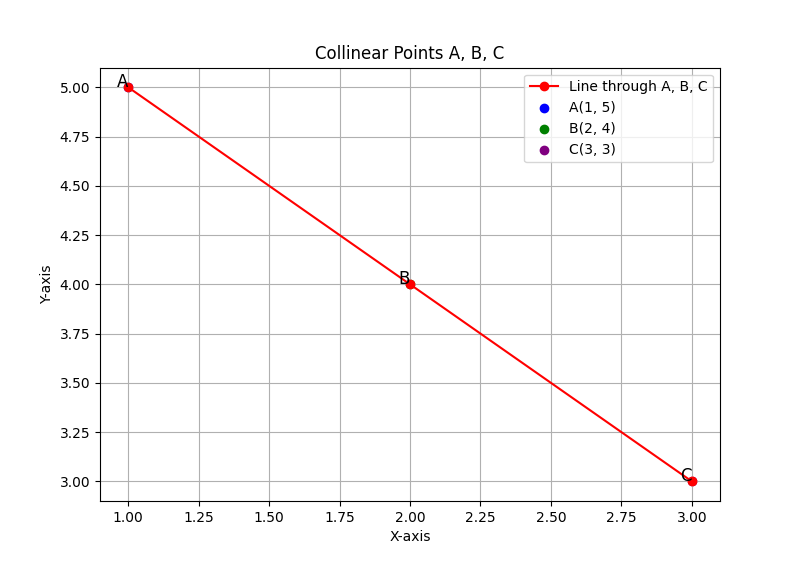
\includegraphics[width=0.7\linewidth]{Figs/Figure_1.jpg}
		\caption{Plot of points $\vec{A}$, $\vec{B}$ and $\vec{C}$}
        \label{stemplot}
\end{figure}
\end{document}
